% =====================================================================
%  Lab 4 -- From Personas & Requirements to Use Cases & UML
%  ZoneSense: Smart Zone Environmental Monitoring and HVAC Control System
% =====================================================================
\documentclass[11pt,a4paper]{article}
% =====================================================================
%  ZoneSense lab reports -- shared preamble
%  CS3151 Software Engineering, Effat University, Fall 2026
%  Compiler: pdfLaTeX (Overleaf default)
% =====================================================================

% ---------- Fonts and encoding ----------
\usepackage[T1]{fontenc}
\usepackage[utf8]{inputenc}
\usepackage{lmodern}               % Latin Modern for typewriter text
\usepackage{mathptmx}              % Times for body text
\usepackage[scaled=0.90]{helvet}   % Helvetica for table headers and captions
\usepackage{textcomp}
\usepackage{amssymb}
\usepackage{microtype}

% ---------- Page layout ----------
\usepackage[a4paper,top=2.2cm,bottom=2.2cm,left=2.2cm,right=2.2cm,headheight=16pt]{geometry}
\setlength{\parindent}{0pt}
\setlength{\parskip}{6pt plus 1pt}
\linespread{1.08}
\setlength{\emergencystretch}{2em}

% ---------- Colours (taken from the SRS) ----------
\usepackage[table]{xcolor}
\definecolor{znavy}{HTML}{173A5E}   % headings, table headers
\definecolor{zteal}{HTML}{1A9EAD}   % sub-headings
\definecolor{zrow}{HTML}{F0F5FA}    % alternating table rows
\definecolor{zline}{HTML}{B7C6D5}   % table rules
\definecolor{znote}{HTML}{FFF6DB}   % call-out background
\definecolor{znotebar}{HTML}{D9A21B}% call-out bar
\definecolor{zpink}{HTML}{FBEDED}
\definecolor{zmint}{HTML}{E3F4F1}
\definecolor{zgreen}{HTML}{1E7B3A}
\definecolor{zcode}{HTML}{F5F7F9}

% ---------- Packages ----------
\usepackage{graphicx}
\usepackage{array}
\usepackage{tabularx}
\usepackage{xltabular}
\usepackage{makecell}
\usepackage{enumitem}
\usepackage{titlesec}
\usepackage{fancyhdr}
\usepackage{float}
\usepackage{caption}
\usepackage{needspace}
\usepackage[most]{tcolorbox}
\usepackage{listings}
\usepackage{xurl}
\usepackage[hidelinks]{hyperref}
\urlstyle{same}

\graphicspath{{figures/}}

% ---------- Headings ----------
\setcounter{secnumdepth}{3}
\titleformat{\section}{\LARGE\bfseries\color{znavy}}{\thesection.}{0.5em}{}
\titleformat{\subsection}{\Large\bfseries\color{zteal}}{\thesubsection}{0.6em}{}
\titleformat{\subsubsection}{\large\bfseries\color{znavy}}{\thesubsubsection}{0.6em}{}
\titleformat{\paragraph}[runin]{\normalsize\bfseries\color{znavy}}{}{0pt}{}
\titlespacing*{\section}{0pt}{6pt}{12pt}
\titlespacing*{\subsection}{0pt}{14pt}{6pt}
\titlespacing*{\subsubsection}{0pt}{12pt}{4pt}
\titlespacing*{\paragraph}{0pt}{8pt}{0.6em}

% ---------- Lists ----------
\setlist{itemsep=2pt,topsep=3pt,parsep=0pt}

% ---------- Tables ----------
\newcolumntype{L}[1]{>{\raggedright\arraybackslash}p{#1}}
\newcolumntype{C}[1]{>{\centering\arraybackslash}p{#1}}
\newcolumntype{Y}{>{\raggedright\arraybackslash}X}
\newcolumntype{B}[1]{>{\raggedright\arraybackslash\leavevmode\bfseries\color{znavy}}p{#1}} % bold navy first column
\newcolumntype{Z}{>{\centering\arraybackslash}X}
\renewcommand{\arraystretch}{1.25}
\setlength{\tabcolsep}{5pt}
\arrayrulecolor{zline}
\newcommand{\hd}[1]{\leavevmode\textcolor{white}{\sffamily\bfseries #1}}   % header cell
\newcommand{\headrow}{\rowcolor{znavy}}                            % header row
\newcommand{\stripe}{\rowcolors{2}{white}{zrow}}                    % zebra rows

% ---------- Captions ----------
\captionsetup{font={small,sf},labelfont={bf,color=znavy},textfont={bf,color=znavy},
  labelsep=endash,justification=raggedright,singlelinecheck=false,skip=4pt}
\captionsetup[figure]{font={small,sf},labelfont={color=gray},textfont={color=gray},
  justification=centering,singlelinecheck=true,skip=6pt}

% ---------- Handy macros ----------
\newcommand{\COtwo}{CO\textsubscript{2}}
\newcommand{\tick}{\ensuremath{\checkmark}}
\newcommand{\gtick}{\textcolor{zgreen}{\ensuremath{\checkmark}}}
\newcommand{\cbox}{\ensuremath{\square}}

% Call-out box (yellow, left bar) -- used for notes in the SRS
\newtcolorbox{zcallout}{enhanced,breakable,colback=znote,colframe=znote,
  borderline west={3pt}{0pt}{znotebar},arc=0pt,outer arc=0pt,
  left=8pt,right=8pt,top=5pt,bottom=5pt,fontupper=\small,before skip=8pt,after skip=8pt}

% Light-blue information box
\newtcolorbox{zinfo}{enhanced,colback=zrow,colframe=zrow,arc=0pt,outer arc=0pt,
  left=8pt,right=8pt,top=6pt,bottom=6pt,fontupper=\small,before skip=8pt,after skip=8pt}

% Code listings
\lstset{basicstyle=\ttfamily\scriptsize,columns=fullflexible,keepspaces=true,
  breaklines=true,breakatwhitespace=false,showstringspaces=false,upquote=true,
  frame=single,rulecolor=\color{zline},backgroundcolor=\color{zcode},
  xleftmargin=4pt,xrightmargin=4pt,framexleftmargin=4pt,framexrightmargin=4pt,
  aboveskip=8pt,belowskip=8pt,tabsize=4,
  literate={≤}{{$\le$}}1 {≥}{{$\ge$}}1 {→}{{$\rightarrow$}}1 {–}{{--}}1}

% ---------- Header and footer ----------
\pagestyle{fancy}
\fancyhf{}
\fancyhead[L]{\small\sffamily\textcolor{znavy}{\ShortTitle}}
\fancyhead[R]{\small\sffamily\textcolor{gray}{CS3151 -- Software Engineering}}
\fancyfoot[L]{\footnotesize\sffamily\textcolor{gray}{CS3151/2026 \quad Dr.\ Passent Elkafrawy}}
\fancyfoot[R]{\footnotesize\sffamily\textcolor{gray}{\thepage}}
\renewcommand{\headrulewidth}{0.4pt}
\renewcommand{\headrule}{\hbox to\headwidth{\color{zline}\leaders\hrule height \headrulewidth\hfill}}

% ---------- Cover page ----------
% Set \LabTitle, \ProjectTitle and \TeamMembers in main.tex before \begin{document}.
\newcommand{\makecover}{%
  \begin{titlepage}
    \centering
    \vspace*{1.2cm}
    
\includegraphics[width=3.6cm]{effat_logo.png}\par
    \vspace{1.6cm}
    {\Large\bfseries Course: CS3151 -- Software Engineering\par}
    \vspace{0.35cm}
    {\large\bfseries Project -- Fall 2026\par}
    \vspace{0.15cm}
    {\large\bfseries Instructor: Dr.\ Passent Elkafrawy\par}
    \vspace{1.6cm}
    {\large\bfseries \ProjectTitle\par}
    \vspace{0.9cm}
    {\color{znavy}\rule{0.55\linewidth}{0.6pt}\par}
    \vspace{0.45cm}
    {\LARGE\bfseries\color{znavy} \LabTitle\par}
    \vspace{0.35cm}
    {\color{znavy}\rule{0.55\linewidth}{0.6pt}\par}
    \vfill
    {\large\bfseries Done By:\par}
    \vspace{0.4cm}
    {\large \TeamMembers\par}
    \vspace{2.2cm}
  \end{titlepage}%
}

% Keep a run-in heading together with the text that follows it
\newcommand{\keephead}[1]{\needspace{6\baselineskip}\paragraph{#1}\leavevmode\par\vspace{-\parskip}}

% Never leave a heading stranded at the bottom of a page
\usepackage{etoolbox}
\pretocmd{\section}{\needspace{8\baselineskip}}{}{}
\pretocmd{\subsection}{\needspace{6\baselineskip}}{}{}
\pretocmd{\subsubsection}{\needspace{5\baselineskip}}{}{}


\newcommand{\ShortTitle}{ZoneSense -- Lab 4: Use Cases \& UML}
\newcommand{\LabTitle}{Lab 4: From Personas \& Requirements\\to Use Cases \& UML}
\newcommand{\ProjectTitle}{ZoneSense: Smart Zone Environmental Monitoring and HVAC Control System}
\newcommand{\TeamMembers}{%
  Remas Rawas --- ID: S24109161\\[6pt]
  Bayan Abduldaym --- ID: S24109196\\[6pt]
  Ghala Bin Salim --- ID: S24109159}

% Shaded, bold first column used in the brief use-case specifications
\newcolumntype{S}[1]{>{\columncolor{zrow}\raggedright\arraybackslash\leavevmode\bfseries\color{znavy}}p{#1}}
% Lists inside table cells
\newenvironment{cellenum}{\begin{minipage}[t]{\linewidth}\begin{enumerate}[nosep,leftmargin=1.6em,label=\arabic*.]}{\end{enumerate}\vspace{2pt}\end{minipage}}
\newenvironment{cellext}{\begin{minipage}[t]{\linewidth}\begin{enumerate}[nosep,leftmargin=2.1em,itemsep=2pt]}{\end{enumerate}\vspace{2pt}\end{minipage}}
% Checklist items
\newcommand{\done}{\raisebox{-1pt}{\fcolorbox{zgreen}{zgreen}{\rule{0pt}{6pt}\makebox[6pt]{\color{white}\scriptsize\boldmath$\checkmark$}}}}
% Use-case diagram figure
\newcommand{\ucfigure}[3][\linewidth]{%
  \begin{figure}[H]\centering
  \includegraphics[width=#1,height=0.62\textheight,keepaspectratio]{#2}
  \caption{#3}\end{figure}}
% Page section headings used throughout this lab
\newcommand{\step}[1]{\section*{#1}\addcontentsline{toc}{section}{#1}}
\newcommand{\substep}[1]{{\large\bfseries\color{zteal}#1\par}\vspace{4pt}}

\begin{document}
\makecover

{\huge\bfseries\color{znavy} Lab 4: From Personas \& Requirements to Use Cases \& UML\par}
\vspace{14pt}

% ---------------------------------------------------------------------
\step{Step 0 -- Warm-up: Extract Actions and Domain Concepts}

\subsection*{Main actions (verbs)}
\begin{itemize}[label=\cbox,itemsep=1pt]
\item Configure monitoring zones
\item Receive and store environmental readings
\item Display current readings and zone status
\item Compare readings with configured thresholds
\item Generate environmental alerts
\item Determine and display a proposed control action
\item Approve or reject a proposed control action
\item Send an approved control command to the external HVAC control system.
\item Continue monitoring after an action or maintenance activity
\item Investigate an environmental incident
\item Record maintenance work and resolution
\item Review zone history
\item Authenticate users and verify role authorization
\item Automatically log system events and timestamps
\end{itemize}

\subsection*{Main domain concepts (nouns)}
\begin{itemize}[label=\cbox,itemsep=1pt]
\item Building
\item Monitoring Zone
\item Environmental Sensor
\item Sensor Reading
\item Temperature / CO2 / Humidity / Sound Level
\item Environmental Status
\item Environmental Alert
\item Control Action
\item Approval Decision
\item Building Resident
\item HVAC Maintenance Technician
\item Maintenance Activity
\item User / Role
\item System Event Log
\end{itemize}

% ---------------------------------------------------------------------
\clearpage
\step{Step 1 -- Identify Actors \& Goals}

{\small\stripe
\begin{xltabular}{\linewidth}{|B{2.6cm}|Y|Y|Y|Y|}
\caption{Actor cards}\label{tab:actors}\\
\hline\headrow
\hd{Actor} & \hd{Description} & \hd{Triggers / Interests} & \hd{Challenges} & \hd{Notes}\\\hline
\endfirsthead
\hline\headrow
\hd{Actor} & \hd{Description} & \hd{Triggers / Interests} & \hd{Challenges} & \hd{Notes}\\\hline
\endhead
Building Resident & Primary operational user who monitors building zones and, when authorized, approves or rejects proposed control actions. & Identify abnormal zones, Review readings and alerts, Approve/reject proposed control actions, Review history & Many readings to monitor, Delayed awareness, Deciding which zone needs attention first & Directly mapped from the Building Resident persona.\\\hline
HVAC Maintenance Technician & Technical user who investigates environmental or HVAC-related incidents and records maintenance activities. & Understand the affected zone, Inspect the issue, Perform maintenance, Document status and resolution & Difficulty locating the source of a problem, Insufficient information before investigation & Directly mapped from the HVAC Maintenance Technician persona.\\\hline
Environmental Sensors & External devices that provide temperature, \COtwo, humidity, and sound-level measurements to the system. & Provide current environmental measurements, Send periodic readings to the system, Support continuous zone monitoring & Sensor failure, Missing readings, Unavailable or inaccurate data & External device actor supporting environmental monitoring.\\\hline
HVAC / Supported Control System & External building-control system that executes approved control actions. & Receive authorized control commands, Execute approved control actions & Must not execute a proposed action before Building Resident approval, Requires reliable communication with the monitoring system & External system actor used only for execution of approved control actions.\\\hline
\end{xltabular}}

\subsection*{Actor goals}

\paragraph{Building Resident:}\leavevmode
\begin{itemize}[label=\cbox,itemsep=1pt]
\item Configure monitoring zones when authorized.
\item Monitor environmental conditions across zones.
\item Identify abnormal conditions and review alert details.
\item Review proposed control actions.
\item Approve or reject proposed control actions when authorized.
\item Monitor the affected zone after an approved action.
\item Review previous alerts, decisions, and executed actions.
\end{itemize}

\paragraph{HVAC Maintenance Technician:}\leavevmode
\begin{itemize}[label=\cbox,itemsep=1pt]
\item Review incident information needed for technical investigation.
\item Identify what requires inspection.
\item Record maintenance work, status, and resolution.
\item Review updated readings after maintenance.
\end{itemize}

\paragraph{Environmental Sensors:}\leavevmode
\begin{itemize}[label=\cbox]
\item Provide current environmental measurements for configured zones.
\end{itemize}

\paragraph{HVAC / Supported Control System:}\leavevmode
\begin{itemize}[label=\cbox]
\item Execute an approved supported control action.
\end{itemize}

\begin{zinfo}
\textbf{\color{znavy}Scope decision.} Building owners remain stakeholders/potential customers, not primary operational actors. The software system itself is the system boundary and is therefore not modeled as an external actor.
\end{zinfo}

% ---------------------------------------------------------------------
\clearpage
\step{Step 2 -- Draft the Use Case List}

{\small\stripe
\begin{xltabular}{\linewidth}{|B{1.2cm}|L{3.3cm}|L{3.4cm}|Y|C{1.5cm}|}
\caption{Prioritized use case list (MoSCoW)}\label{tab:uclist}\\
\hline\headrow
\hd{ID} & \hd{Use Case Name} & \hd{Primary Actor / Initiator} & \hd{Goal / Outcome} & \hd{Priority}\\\hline
\endfirsthead
\hline\headrow
\hd{ID} & \hd{Use Case Name} & \hd{Primary Actor / Initiator} & \hd{Goal / Outcome} & \hd{Priority}\\\hline
\endhead
UC-1 & Configure ZoneSense System & Building Resident & Configure monitoring zones and environmental thresholds for accurate monitoring. & Must\\\hline
UC-2 & Monitor Building Zones & Building Resident (Supporting: Environmental Sensors) & Receive environmental readings and display current zone conditions and statuses. & Must\\\hline
UC-3 & Manage Environmental Alerts & Building Resident & Review environmental alerts and proposed control actions, then approve or reject supported actions. & Must\\\hline
UC-4 & Execute Approved Control Action & HVAC / Supported Control System & Execute an approved control command and return the execution result to ZoneSense. & Must\\\hline
UC-5 & Review Zone History & Building Resident & Review previous readings, alerts, decisions, and control actions for a selected zone. & Should\\\hline
UC-6 & Document Maintenance Activities & HVAC Maintenance Technician & Investigate environmental incidents and record maintenance work, status, and resolution. & Must\\\hline
\end{xltabular}}

\subsection*{Traceability to Finalized Lab 3 Requirements}

\newcommand{\uch}[3]{\hd{\makebox[\linewidth]{\scriptsize\makecell[t]{#1\\#2\\#3}}}}
\newcommand{\mhead}{\hline\headrow
\hd{Requirement} & \uch{UC-1}{Configure}{ZoneSense} & \uch{UC-2}{Monitor}{Zones} & \uch{UC-3}{Manage}{Alerts} & \uch{UC-4}{Execute}{Action} & \uch{UC-5}{Review}{History} & \uch{UC-6}{Mainte-}{nance} & \hd{Reason}\\\hline}
{\footnotesize\stripe\setlength{\tabcolsep}{3pt}
\begin{xltabular}{\linewidth}{|L{3.3cm}|C{1.3cm}|C{1.3cm}|C{1.3cm}|C{1.3cm}|C{1.3cm}|C{1.3cm}|Y|}
\caption{Traceability matrix: requirements to use cases}\label{tab:trace}\\
\mhead
\endfirsthead
\mhead
\endhead
FR1 -- Configure up to 20 zones & \gtick & & & & & & Supports zone configuration.\\\hline
FR2 -- Receive 4 measurements every 60 sec & & \gtick & & & & & Supports continuous sensor monitoring.\\\hline
FR3 -- Store sensor readings & & \gtick & & & & & Supports monitoring data storage.\\\hline
FR4 -- Display current readings within 8 sec & & \gtick & & & & & Supports current zone monitoring.\\\hline
FR5 -- Compare readings with thresholds & & \gtick & & & & & Supports threshold evaluation.\\\hline
FR6 -- Display zone status & & \gtick & & & & & Supports zone-status monitoring.\\\hline
FR7 -- Generate abnormal-condition alert & & & \gtick & & & & Supports alert handling.\\\hline
FR8 -- Alert contains zone, reading and severity & & & \gtick & & & & Supports complete alert review.\\\hline
FR9 -- Propose supported control action & & & \gtick & & & & Supports control-action proposal.\\\hline
FR10 -- Require approval before execution & & & \gtick & \gtick & & & UC3 approves; UC4 verifies before execution.\\\hline
FR11 -- Approve/reject proposed action & & & \gtick & & & & Supports approval and rejection.\\\hline
FR12 -- Send approved action to control system & & & & \gtick & & & Supports approved action execution.\\\hline
FR13 -- Reject proposed control action & & & \gtick & & & & UC3 records rejection and prevents execution\\\hline
FR14 -- Record approval/rejection decision & & & \gtick & & & & UC3 records the decision for traceability\\\hline
FR15 -- Continue monitoring after action/maintenance & & \gtick & & \gtick & & & UC2 continues monitoring; UC4 continues after execution.\\\hline
FR16 -- Display incident information & & & & & & \gtick & UC6 provides the technician with incident details\\\hline
FR17 -- Record maintenance work and resolution & & & & & & \gtick & UC6 records maintenance work, status, and resolution\\\hline
FR18 -- Store alerts, decisions, actions, and maintenance records & & & \gtick & \gtick & \gtick & \gtick & These use cases create or use stored operational records.\\\hline
FR19 -- Retrieve zone history & & & & & \gtick & & Supports historical record access.\\\hline
FR20 -- Require authentication & \gtick & & \gtick & \gtick & \gtick & \gtick & Protects configuration, alerts, actions, history, maintenance.\\\hline
FR21 -- Verify user role & \gtick & & \gtick & \gtick & \gtick & \gtick & Controls access across protected use cases.\\\hline
FR22 -- Suppress repeat alerts & \gtick & & \gtick & & & & Used by UC1 to set the interval and UC3 to suppress repeats.\\\hline
NFR1 -- Performance & & \gtick & & & & & Used by UC2 for monitoring updates.\\\hline
NFR2 -- Alert response time & & & \gtick & & & & Used by UC3 for timely alerts.\\\hline
NFR3 -- Availability & & \gtick & & \gtick & \gtick & & Used by UC2 for sensor availability.\\\hline
NFR4 -- Security & \gtick & \gtick & \gtick & \gtick & \gtick & \gtick & Used by all protected use cases.\\\hline
NFR5 -- Authorization & \gtick & \gtick & \gtick & \gtick & \gtick & \gtick & Used by all role-based use cases.\\\hline
NFR6 -- Auditability & & & \gtick & \gtick & \gtick & \gtick & Used by UC3--UC6 for traceability.\\\hline
NFR7 -- Data integrity & & \gtick & & & & & Used by UC2 for stored readings.\\\hline
NFR8 -- Reliability & & \gtick & & & & & Used by UC2 for continuous monitoring.\\\hline
NFR9 -- Usability & & \gtick & & & & & Used by UC2 for status display.\\\hline
NFR10 -- Privacy & & \gtick & & & & & Used by UC2 for sound monitoring.\\\hline
NFR11 -- Maintainability & \gtick & & & & & & Used by UC1 for configuration changes.\\\hline
NFR12 -- Scalability & \gtick & \gtick & & & & & Used by UC1 and UC2 for scale.\\\hline
NFR13 -- Transport security & \gtick & \gtick & \gtick & \gtick & \gtick & \gtick & Used by all use cases for encrypted communication.\\\hline
\end{xltabular}}

% ---------------------------------------------------------------------
\clearpage
\step{Step 3A -- Brief Use Case Specifications}

{\footnotesize\stripe
\begin{xltabular}{\linewidth}{|B{2.4cm}|L{2.5cm}|Y|Y|Y|}
\caption{Brief use case specifications}\label{tab:brief}\\
\hline\headrow
\hd{Use Case} & \hd{Primary Actor / Initiator} & \hd{Preconditions} & \hd{Postconditions} & \hd{Main Success Scenario (1--2 lines)}\\\hline
\endfirsthead
\hline\headrow
\hd{Use Case} & \hd{Primary Actor / Initiator} & \hd{Preconditions} & \hd{Postconditions} & \hd{Main Success Scenario (1--2 lines)}\\\hline
\endhead
UC-1 Configure ZoneSense System & Building Resident & Building Resident is authenticated and authorized; the building exists. & Zone configuration, environmental thresholds and repeat-alert intervals are saved and available for monitoring. & Building Resident creates or updates monitoring zones, thresholds and repeat-alert intervals; ZoneSense validates and saves the configuration.\\\hline
UC-2 Monitor Building Zones & Building Resident; Environmental Sensors & Zones are configured; sensors are connected or their data is marked unavailable; Building Resident is authenticated. & Received readings are stored, and current measurements and zone statuses are displayed. & Sensors provide environmental readings; ZoneSense receives, stores, and evaluates them, then displays current measurements and statuses to the Building Resident.\\\hline
UC-3 Manage Environmental Alerts & Building Resident & An environmental alert exists; Building Resident is authenticated and authorized. & Alert details and any supported proposed action are displayed; the approval or rejection decision is recorded. & Building Resident reviews an alert and any proposed control action, then approves or rejects the proposal when applicable.\\\hline
UC-4 Execute Approved Control Action & HVAC / Supported Control System (external; acts only on a recorded approval) & A supported control action has been approved by the Building Resident, and the approval is recorded. & The execution result is received and recorded; monitoring continues for the affected zone. & ZoneSense sends the approved command to the HVAC control system, which executes it and returns the execution result.\\\hline
UC-5 Review Zone History & Building Resident & Building Resident is authenticated and authorized; the selected zone has historical records. & Previous alerts, approval decisions, and executed control actions are displayed. & Building Resident selects a zone and requests its history; ZoneSense retrieves and displays the associated records.\\\hline
UC-6 Document Maintenance Activities & HVAC Maintenance Technician & Technician is authenticated and authorized; an environmental incident exists. & Submitted maintenance work, status, and resolution outcome are stored. & Technician reviews incident details, investigates the problem, and records the maintenance work, status, and whether the issue was resolved.\\\hline
\end{xltabular}}

% ---------------------------------------------------------------------
\clearpage
\step{Step 4 -- Overall Use Case Diagram}
\substep{All use cases and actors}
\ucfigure{uc_overall.png}{Overall use case diagram}
All six use cases connect to an actor (Building Resident, HVAC Maintenance Technician, Environmental Sensors, HVAC / supported control system) or to another use case through \guillemotleft extend\guillemotright. Every use case includes authentication and role verification (FR20, FR21, NFR4, NFR5); these included steps are shown in the detailed diagrams.

% ---------------------------------------------------------------------
\clearpage
\step{UC-1: Configure ZoneSense System}
\substep{Brief use case specification and use case diagram}
{\small
\begin{tabularx}{\linewidth}{|S{4cm}|Y|}\hline
Primary actor / initiator & Building Resident\\\hline
Preconditions & Building Resident is authenticated and authorized; the building exists.\\\hline
Postconditions & Zone configuration and environmental thresholds are saved and available for monitoring.\\\hline
Main success scenario & Building Resident creates or updates monitoring zones, thresholds and repeat-alert intervals; ZoneSense validates and saves the configuration.\\\hline
\end{tabularx}}
\ucfigure{uc1.png}{UC-1 -- Configure ZoneSense System}

% ---------------------------------------------------------------------
\clearpage
\step{Step 3B -- Fully Dressed Use Case: UC-2 Monitor Building Zones}

{\small\stripe
\begin{xltabular}{\linewidth}{|B{4.2cm}|Y|}
\caption{Fully dressed use case: UC-2 Monitor Building Zones}\label{tab:uc2}\\
\hline\headrow \hd{Field} & \hd{Content}\\\hline
\endfirsthead
\hline\headrow \hd{Field} & \hd{Content}\\\hline
\endhead
Use Case & UC-2 --- Monitor Building Zones\\\hline
Activity Name & Monitor Building Zones\\\hline
Primary Actor & Building Resident\\\hline
Supporting Actor & Environmental Sensors\\\hline
Stakeholders \& Interests & Building Resident: needs a clear and current view of environmental conditions. Occupants/organization: need safe, comfortable, and traceable monitoring.\\\hline
Preconditions & The Building Resident is authenticated and authorized. Monitoring zones are configured. Sensor data is available or its absence can be detected.\\\hline
Postconditions & The system displays the most recent temperature, \COtwo, humidity, and sound-level readings and exactly one current status (normal, warning, critical, or unavailable) for each monitored zone.\\\hline
Main Success Scenario (Flow of Control) & \begin{cellenum}
\item Building Resident opens the building monitoring view.
\item ZoneSense obtains the most recently received readings for each zone.
\item ZoneSense compares the readings with configured thresholds.
\item ZoneSense determines the current zone status.
\item ZoneSense displays the four environmental measurements and the zone status.
\item Building Resident identifies zones that require attention.
\end{cellenum}\\\hline
Extensions / Alternatives & \begin{cellext}
\item[2a.] A sensor misses 3 consecutive 60-second reporting intervals $\rightarrow$ its data is marked unavailable and the affected zone reflects the unavailable condition.
\item[3a.] A reading violates a configured threshold $\rightarrow$ ZoneSense generates an environmental alert, which may lead to UC-3: Manage Environmental Alerts.
\end{cellext}\\\hline
Special Requirements & Monitoring interface update $\leq$ 8 seconds after new data. Functioning sensor measurements are received at least once every 60 seconds. Status changes are displayed within 8 seconds. One sensor failure must not stop other functioning sensor/zone data.\\\hline
Constraints & Single-building scope; up to 20 monitoring zones and 4 environmental measurement types per zone (up to 80 measurement streams). Sound monitoring stores sound-level values only, not audio conversations.\\\hline
Open Issues & Exact threshold values are not fixed in the current project documents; they remain authorized configuration values.\\\hline
\end{xltabular}}

% ---------------------------------------------------------------------
\clearpage
\step{Step 4 -- Use Case Diagram: UC-2 Monitor Building Zones}
\substep{UC-2}
\ucfigure{uc2.png}{UC-2 -- Monitor Building Zones}
Requirements: FR2--FR6, NFR1, NFR3, NFR8, NFR9. Environmental Sensors supply the readings.

% ---------------------------------------------------------------------
\clearpage
\step{Step 3B -- Fully Dressed Use Case: UC-3 Manage Environmental Alerts}

{\small\stripe
\begin{xltabular}{\linewidth}{|B{4.2cm}|Y|}
\caption{Fully dressed use case: UC-3 Manage Environmental Alerts}\label{tab:uc3}\\
\hline\headrow \hd{Field} & \hd{Content}\\\hline
\endfirsthead
\hline\headrow \hd{Field} & \hd{Content}\\\hline
\endhead
Use Case & UC-3 --- Manage Environmental Alerts\\\hline
Activity Name & Manage Environmental Alerts\\\hline
Primary Actor & Building Resident\\\hline
Supporting Actor & None\\\hline
Stakeholders \& Interests & Building Resident: needs to identify abnormal conditions and make safe control decisions. Occupants/organization: need timely alerts and controlled responses to environmental problems.\\\hline
Preconditions & An environmental alert has been generated. The Building Resident is authenticated and authorized.\\\hline
Postconditions & The alert and any supported proposed control action are displayed. The Building Resident's approval or rejection decision is recorded. No control action is executed without recorded approval.\\\hline
Main Success Scenario (Flow of Control) & \begin{cellenum}
\item Building Resident opens and reviews an existing environmental alert.
\item ZoneSense displays a supported proposed HVAC action, if available.
\item Building Resident reviews the proposal.
\item Building Resident approves the proposed action.
\item ZoneSense records the approval decision.
\item The approved action becomes eligible for UC-4: Execute Approved Control Action.
\end{cellenum}\\\hline
Extensions / Alternatives & \begin{cellext}
\item[2a.] No supported HVAC action is available $\rightarrow$ ZoneSense displays the alert without a control proposal; the incident remains available for investigation.
\item[4a.] Building Resident rejects the proposal $\rightarrow$ ZoneSense records the rejection and does not authorize execution.
\item[1a.] The same condition recurs with unchanged severity inside the configured repeat-alert interval $\rightarrow$ ZoneSense stores the repeat in the alert history and does not display a new alert (FR22).
\end{cellext}\\\hline
Special Requirements & Alerts are generated and displayed within 45 seconds of detecting a threshold violation. Supported control proposals are displayed within 10 seconds of identifying a controllable abnormal condition. Approval or rejection decisions are recorded.\\\hline
Constraints & Only an authorized Building Resident can approve or reject proposed control actions. ZoneSense must not send an unapproved control command to the HVAC system.\\\hline
Open Issues & Exact environmental thresholds and the list of supported HVAC control actions require configuration and confirmation.\\\hline
\end{xltabular}}

% ---------------------------------------------------------------------
\clearpage
\step{Step 4 -- Use Case Diagram: UC-3 Manage Environmental Alerts}
\substep{UC-3}
\ucfigure{uc3.png}{UC-3 -- Manage Environmental Alerts}
Requirements: FR7--FR14, FR22, NFR2, NFR6.

% ---------------------------------------------------------------------
\clearpage
\step{Step 5A -- Activity Diagram for UC-3: Manage Environmental Alerts}
\begin{figure}[H]\centering
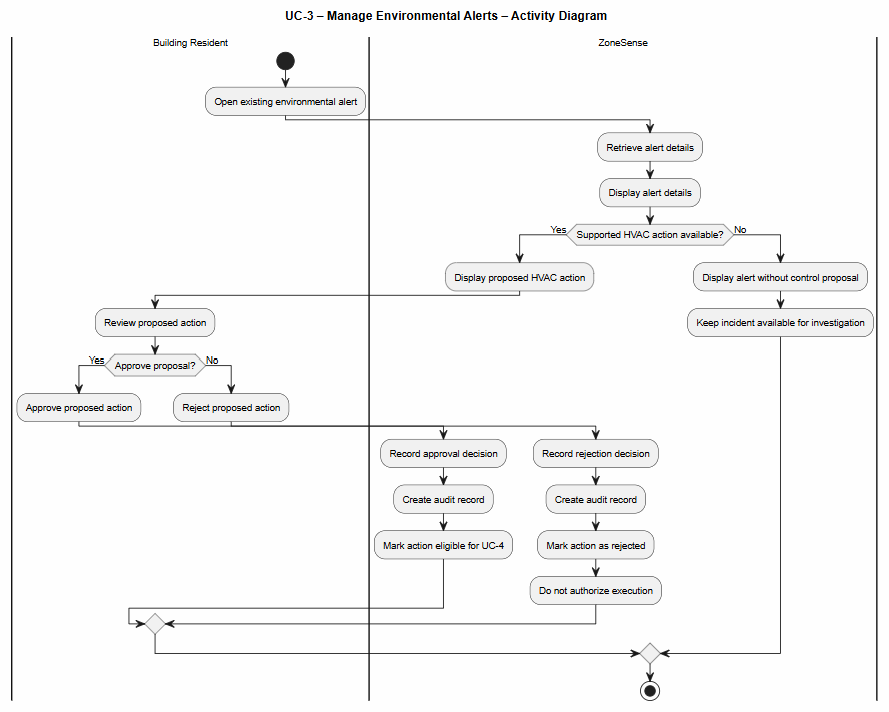
\includegraphics[width=\linewidth,height=0.78\textheight,keepaspectratio]{uc3_activity.png}
\caption{UC-3 -- Manage Environmental Alerts -- Activity Diagram}
\end{figure}

% ---------------------------------------------------------------------
\clearpage
\step{Step 5B -- Sequence Diagram for UC-3: Manage Environmental Alerts}
\substep{Sequence Diagram for the Main Success Scenario}
\begin{figure}[H]\centering
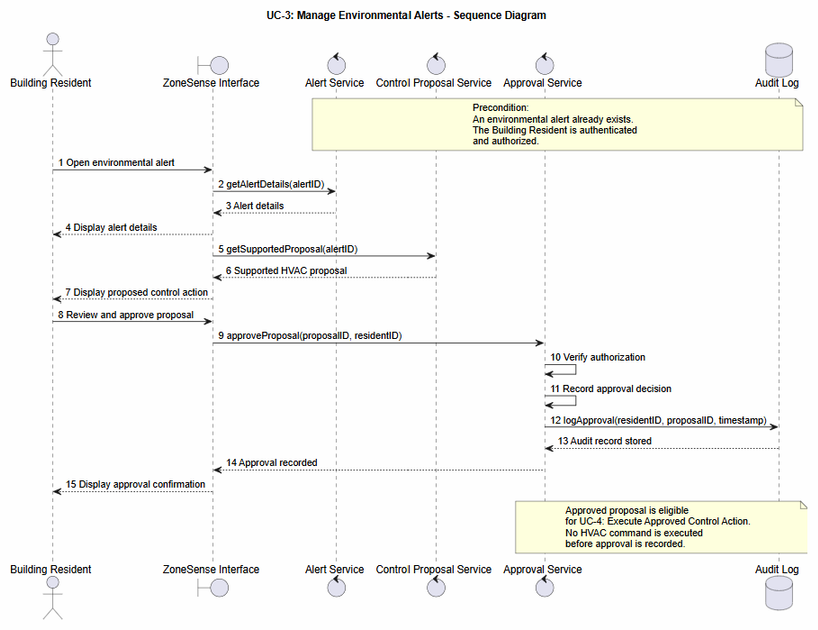
\includegraphics[width=\linewidth,height=0.78\textheight,keepaspectratio]{uc3_sequence.png}
\caption{UC-3: Manage Environmental Alerts -- Sequence Diagram}
\end{figure}

% ---------------------------------------------------------------------
\clearpage
\step{Bonus 2 -- System Sequence Diagram: UC-3 Rejected Control Action (+5 Points)}
\begin{figure}[H]\centering
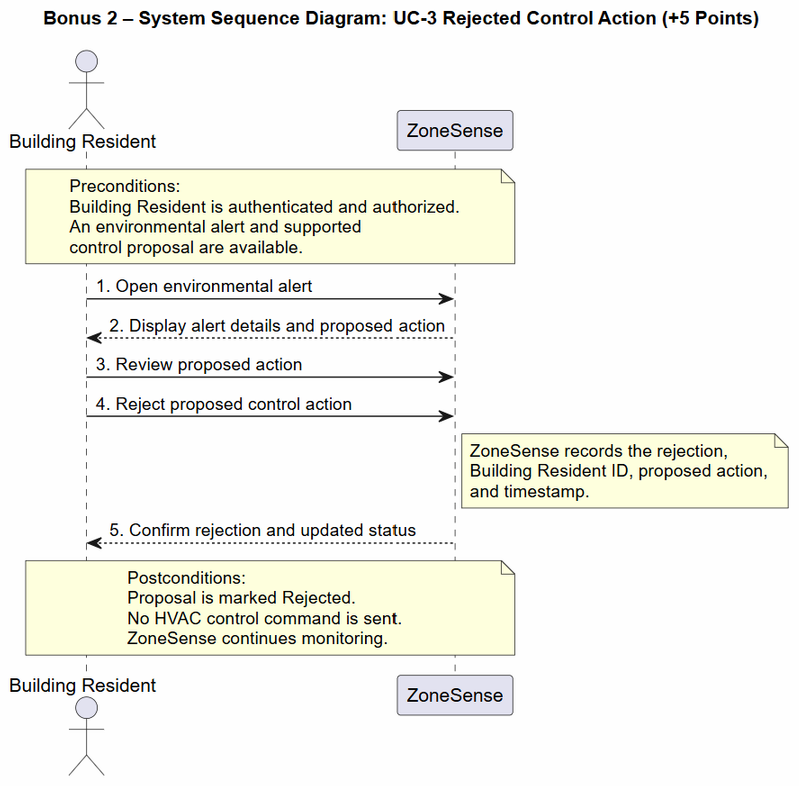
\includegraphics[width=0.92\linewidth,height=0.78\textheight,keepaspectratio]{uc3_rejected_ssd.png}
\caption{System sequence diagram: UC-3 rejected control action}
\end{figure}

% ---------------------------------------------------------------------
\clearpage
\step{UC-4: Execute Approved Control Action}
\substep{Brief use case specification and use case diagram}
{\small
\begin{tabularx}{\linewidth}{|S{4cm}|Y|}\hline
Primary actor / trigger & Building Resident; execution is triggered when an authorized approval is recorded.\\\hline
Supporting actor & HVAC / Supported Control System (external); receives the approved command and returns the execution result.\\\hline
Preconditions & A supported control action has been approved by the Building Resident, and the approval is recorded.\\\hline
Postconditions & The execution result is received and recorded; monitoring continues for the affected zone.\\\hline
Main success scenario & ZoneSense sends the approved command to the HVAC control system, which executes it and returns the execution result.\\\hline
\end{tabularx}}
\ucfigure{uc4.png}{UC-4 -- Execute Approved Control Action}

% ---------------------------------------------------------------------
\clearpage
\step{Additional Diagrams}
State machine of the control-action lifecycle and a system sequence diagram for an alternative flow (rejected control action).

\subsection*{Bonus 1 -- State Machine Diagram: Control Action Lifecycle (+5 Points)}
\begin{figure}[H]\centering
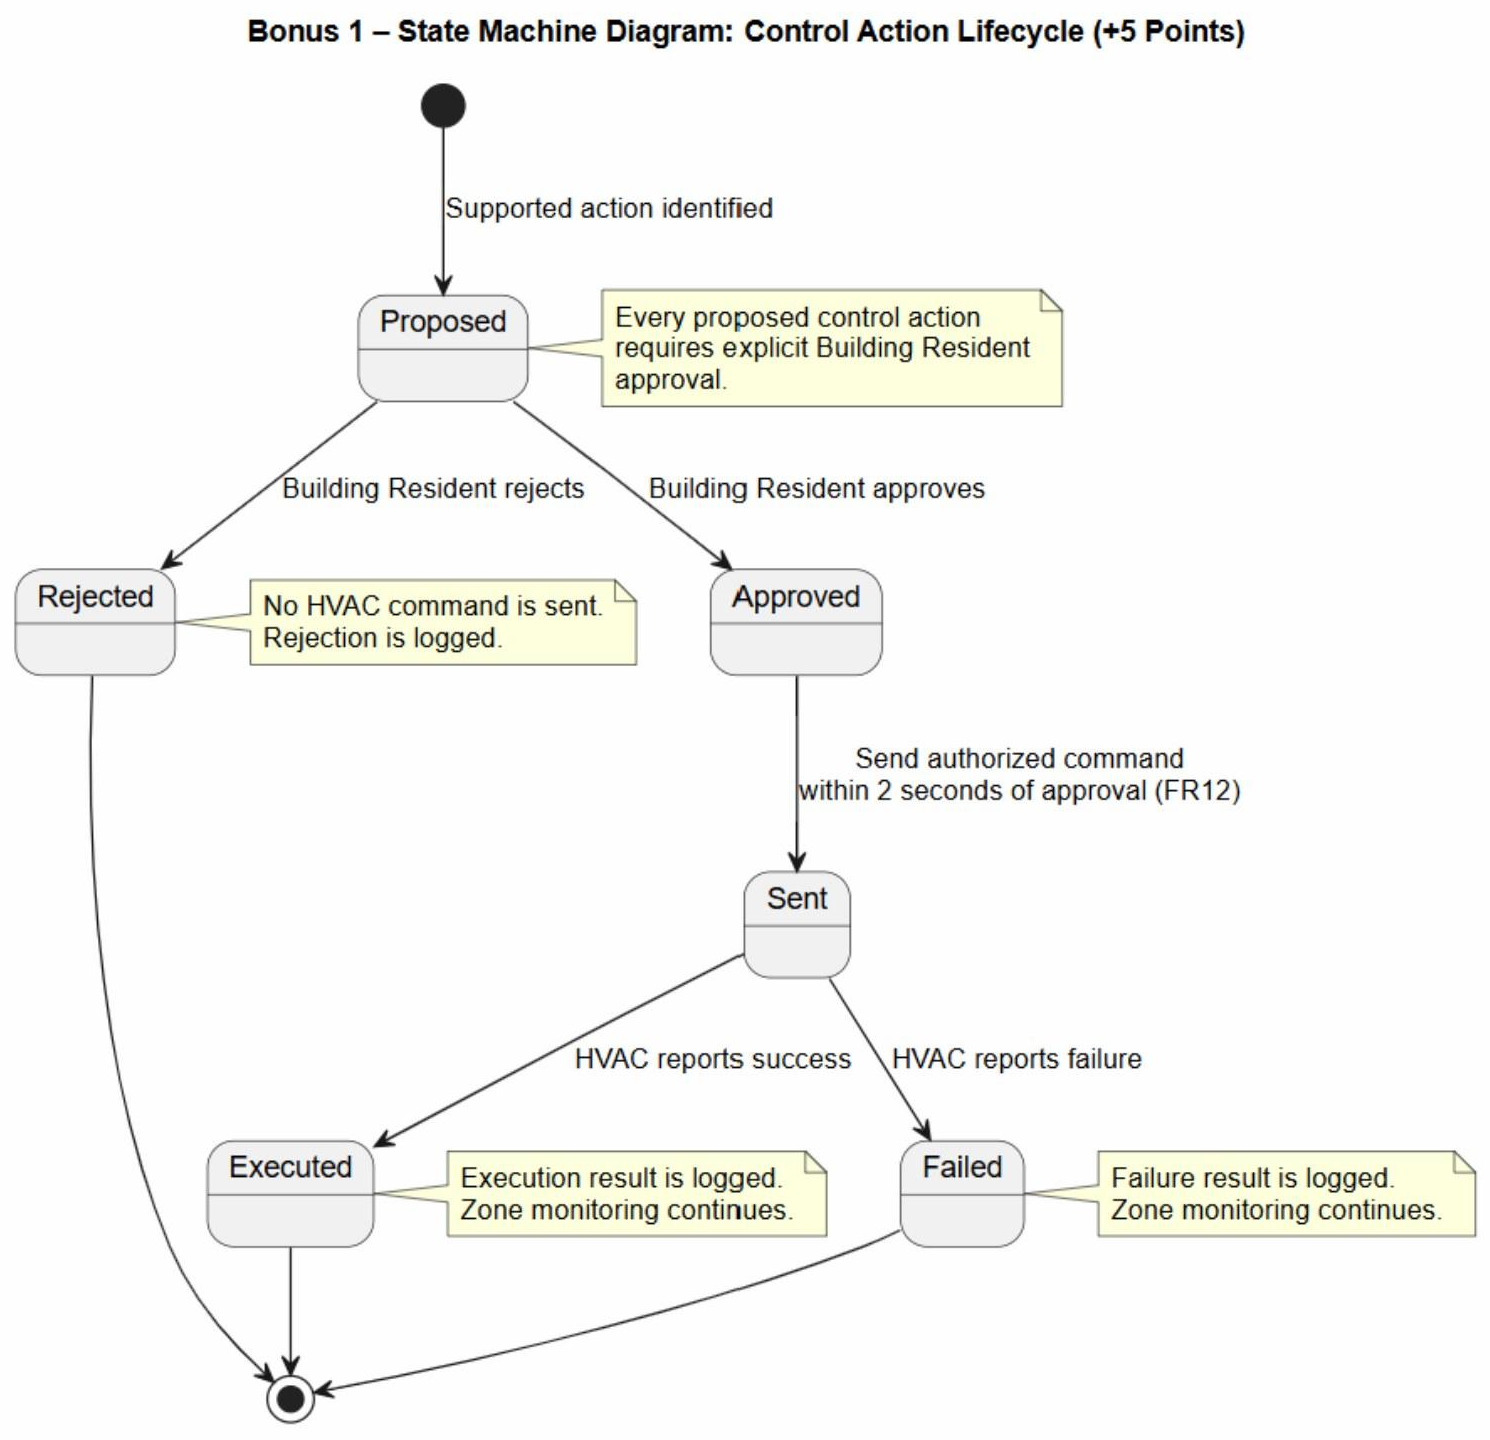
\includegraphics[width=0.92\linewidth,height=0.7\textheight,keepaspectratio]{state_machine.png}
\caption{State machine diagram: control action lifecycle}
\end{figure}

% ---------------------------------------------------------------------
\clearpage
\step{UC-5: Review Zone History}
\substep{Brief use case specification and use case diagram}
{\small
\begin{tabularx}{\linewidth}{|S{4cm}|Y|}\hline
Primary actor / initiator & Building Resident\\\hline
Preconditions & Building Resident is authenticated and authorized; the selected zone has historical records.\\\hline
Postconditions & Previous alerts, approval decisions, and executed control actions are displayed.\\\hline
Main success scenario & Building Resident selects a zone and requests its history; ZoneSense retrieves and displays the associated records.\\\hline
\end{tabularx}}
\ucfigure{uc5.png}{UC-5 -- Review Zone History}

% ---------------------------------------------------------------------
\clearpage
\step{UC-6: Document Maintenance Activities}
\substep{Brief use case specification and use case diagram}
{\small
\begin{tabularx}{\linewidth}{|S{4cm}|Y|}\hline
Primary actor / initiator & HVAC Maintenance Technician\\\hline
Preconditions & Technician is authenticated and authorized; an environmental incident exists.\\\hline
Postconditions & Submitted maintenance work, status, and resolution outcome are stored.\\\hline
Main success scenario & Technician reviews incident details, investigates the problem, and records the maintenance work, status, and whether the issue was resolved.\\\hline
\end{tabularx}}
\ucfigure{uc6.png}{UC-6 -- Document Maintenance Activities}

% ---------------------------------------------------------------------
\clearpage
\step{Step 6 -- Domain Model (Class Diagram)}
Entities shared by use cases UC-1 to UC-6. ThresholdSetting holds the configured limits and repeat-alert interval (FR5, FR22, NFR11); SuppressedRepeat stores repeats that were not re-notified (FR22).
\begin{figure}[H]\centering
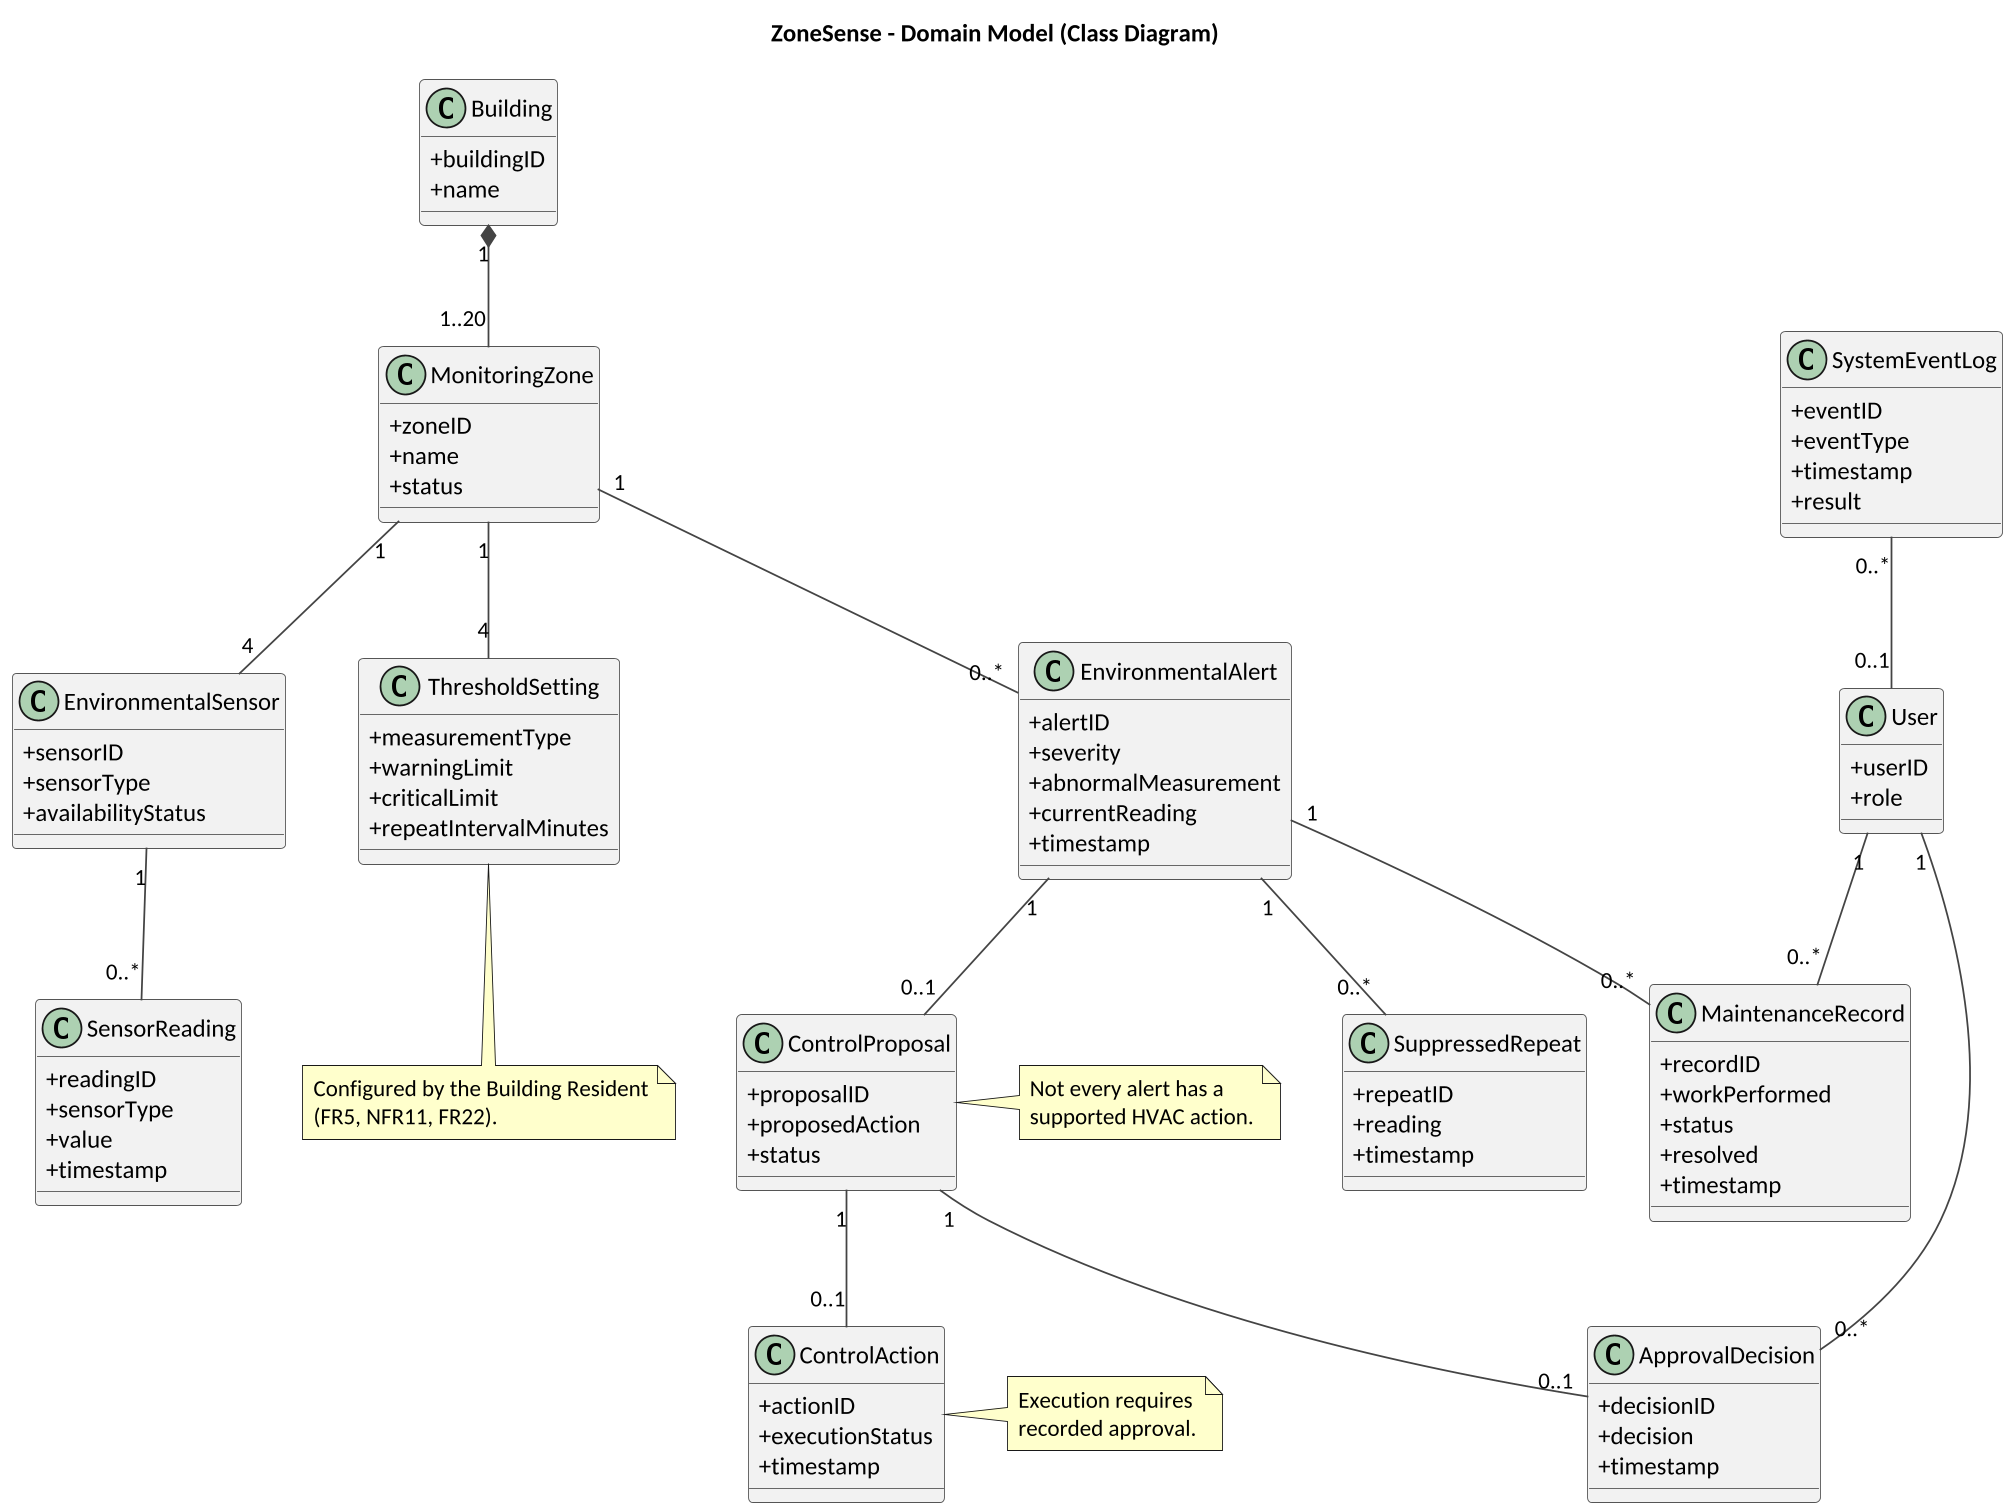
\includegraphics[width=\linewidth,height=0.72\textheight,keepaspectratio]{domain_model.png}
\caption{ZoneSense -- Domain Model (Class Diagram)}
\end{figure}

% ---------------------------------------------------------------------
\clearpage
\step{Step 7 -- Consistency Checks}

{\small\stripe
\begin{xltabular}{\linewidth}{|B{5cm}|Y|}
\caption{Consistency checks}\label{tab:consistency}\\
\hline\headrow \hd{Consistency Check} & \hd{Verification}\\\hline
\endfirsthead
\hline\headrow \hd{Consistency Check} & \hd{Verification}\\\hline
\endhead
Actor and Use Case Traceability & All six use cases (UC-1 to UC-6) are linked to external actors and represented in the overall and individual use case diagrams.\\\hline
Sequence Diagram Alignment & The UC-3 sequence diagram aligns with its main success scenario, with automatic alert detection shown as preliminary system behavior.\\\hline
Activity Diagram Alignment & The UC-3 activity diagram covers supported and unsupported control proposals, approval or rejection, and eligibility for UC-4.\\\hline
Domain Class Consistency & Core domain entities support monitoring, alerts, control actions, approval decisions, and maintenance activities across UC-1 to UC-6.\\\hline
Non-Functional Requirements & Relevant performance, security, availability, privacy, auditability, and scalability constraints are documented in the UML artifacts.\\\hline
\end{xltabular}}

\vspace{10pt}
\step{Step 8 -- Peer Review Sheet}
\begin{itemize}[label=\done,itemsep=4pt,leftmargin=2em]
\item Actors cover all personas and external systems
\item Use case names are goal-level and unambiguous
\item Includes/extends used sparingly and correctly
\item Activity/Sequence diagrams match narratives
\item Class diagram avoids UI/DB details; multiplicities make sense
\item Clear pre/post-conditions and success guarantees
\item Consistency across all artifacts
\item Clarity, readability, and professional style
\end{itemize}

\end{document}
